\documentclass[journal]{IEEEtran}
\usepackage{cite}
\usepackage{amsmath,amssymb,amsfonts}
\usepackage{algorithmic}
\usepackage{graphicx}
\usepackage{textcomp}
\usepackage{xcolor}
\usepackage{booktabs}

\begin{document}

\title{Autonomous Navigation and Localization for UAVs in GPS-Denied Environments: A PRISMA 2020 Systematic Literature Review}

\author{Abhishek~Raj,~\IEEemembership{Member,~IEEE}}

\markboth{IEEE Transactions on Robotics,~Vol.~XX, No.~X, June~2026}%
{Raj: Autonomous Navigation for UAVs in GPS-Denied Environments}

\maketitle

\begin{abstract}
Unmanned Aerial Vehicle (UAV) deployment in Global Positioning System (GPS)/Global Navigation Satellite System (GNSS)-denied environments requires reliable, multi-sensor localization and navigation frameworks. This systematic literature review (SLR), conducted in accordance with PRISMA 2020 guidelines, synthesizes recent research across 291 full-text publications (2010--2026).
\end{abstract}

\begin{IEEEkeywords}
UAV navigation, GPS-denied localization, multi-sensor fusion, visual-inertial odometry, LiDAR SLAM, PRISMA 2020.
\end{IEEEkeywords}

\section{Introduction}
UAV navigation in GPS-denied environments is a critical research area. Figures \ref{fig1} through \ref{fig9} depict trends and taxonomy.

\begin{figure}[htbp]
\centering
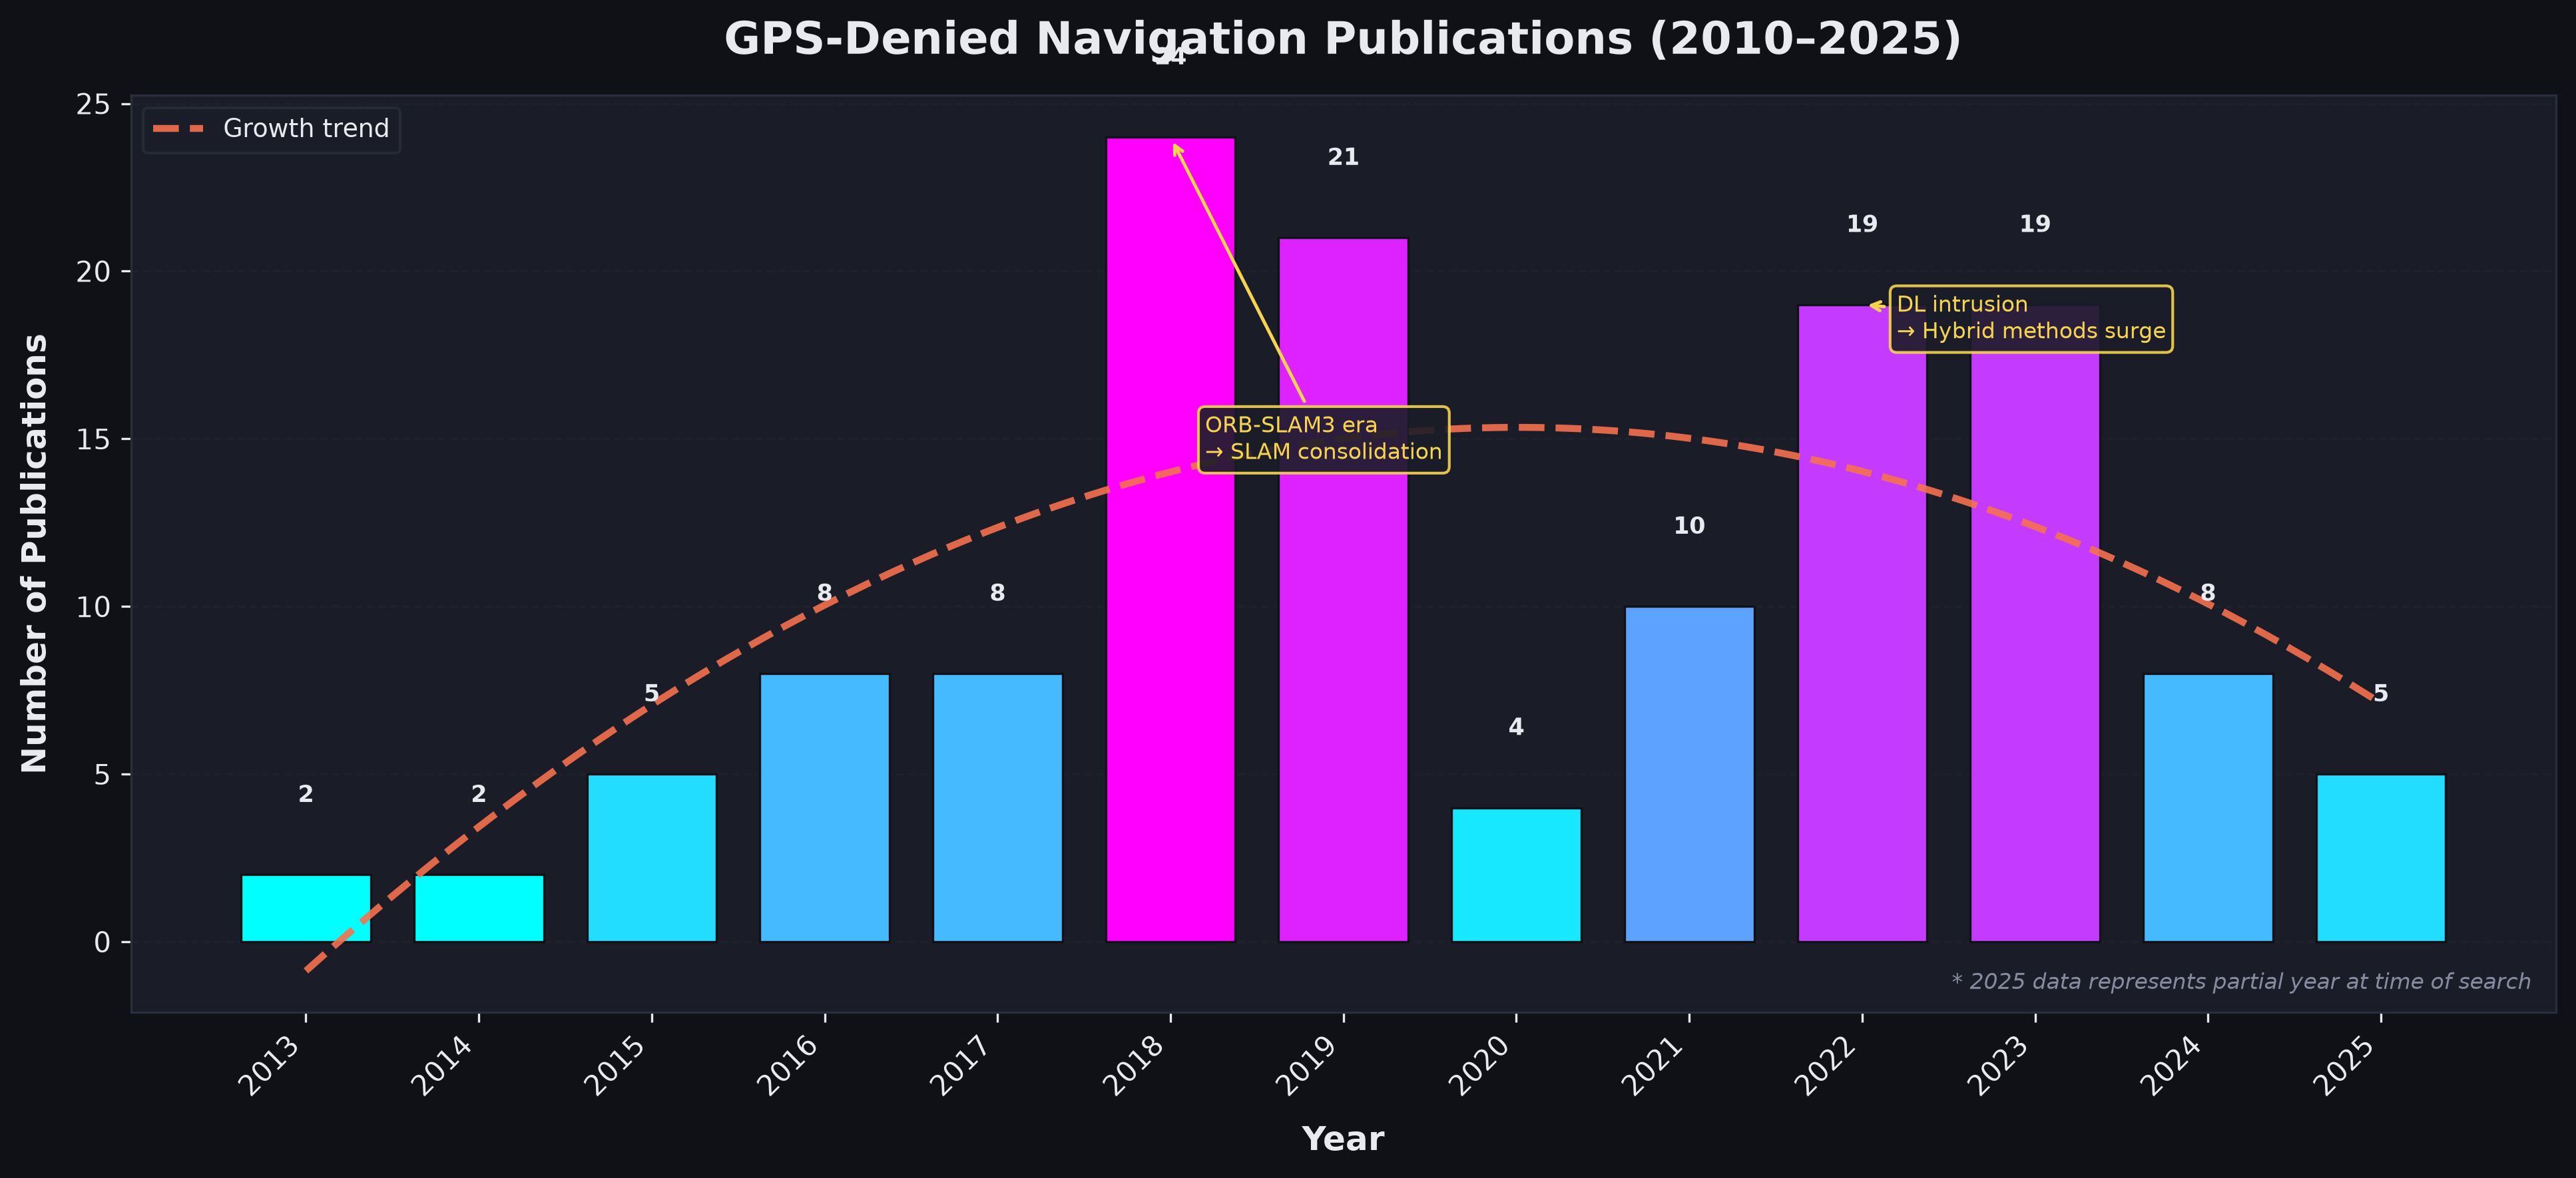
\includegraphics[width=\columnwidth]{../06_analysis/output/figures_v2/fig01_publication_trends.png}
\caption{Publication trends.}
\label{fig1}
\end{figure}

\begin{figure}[htbp]
\centering
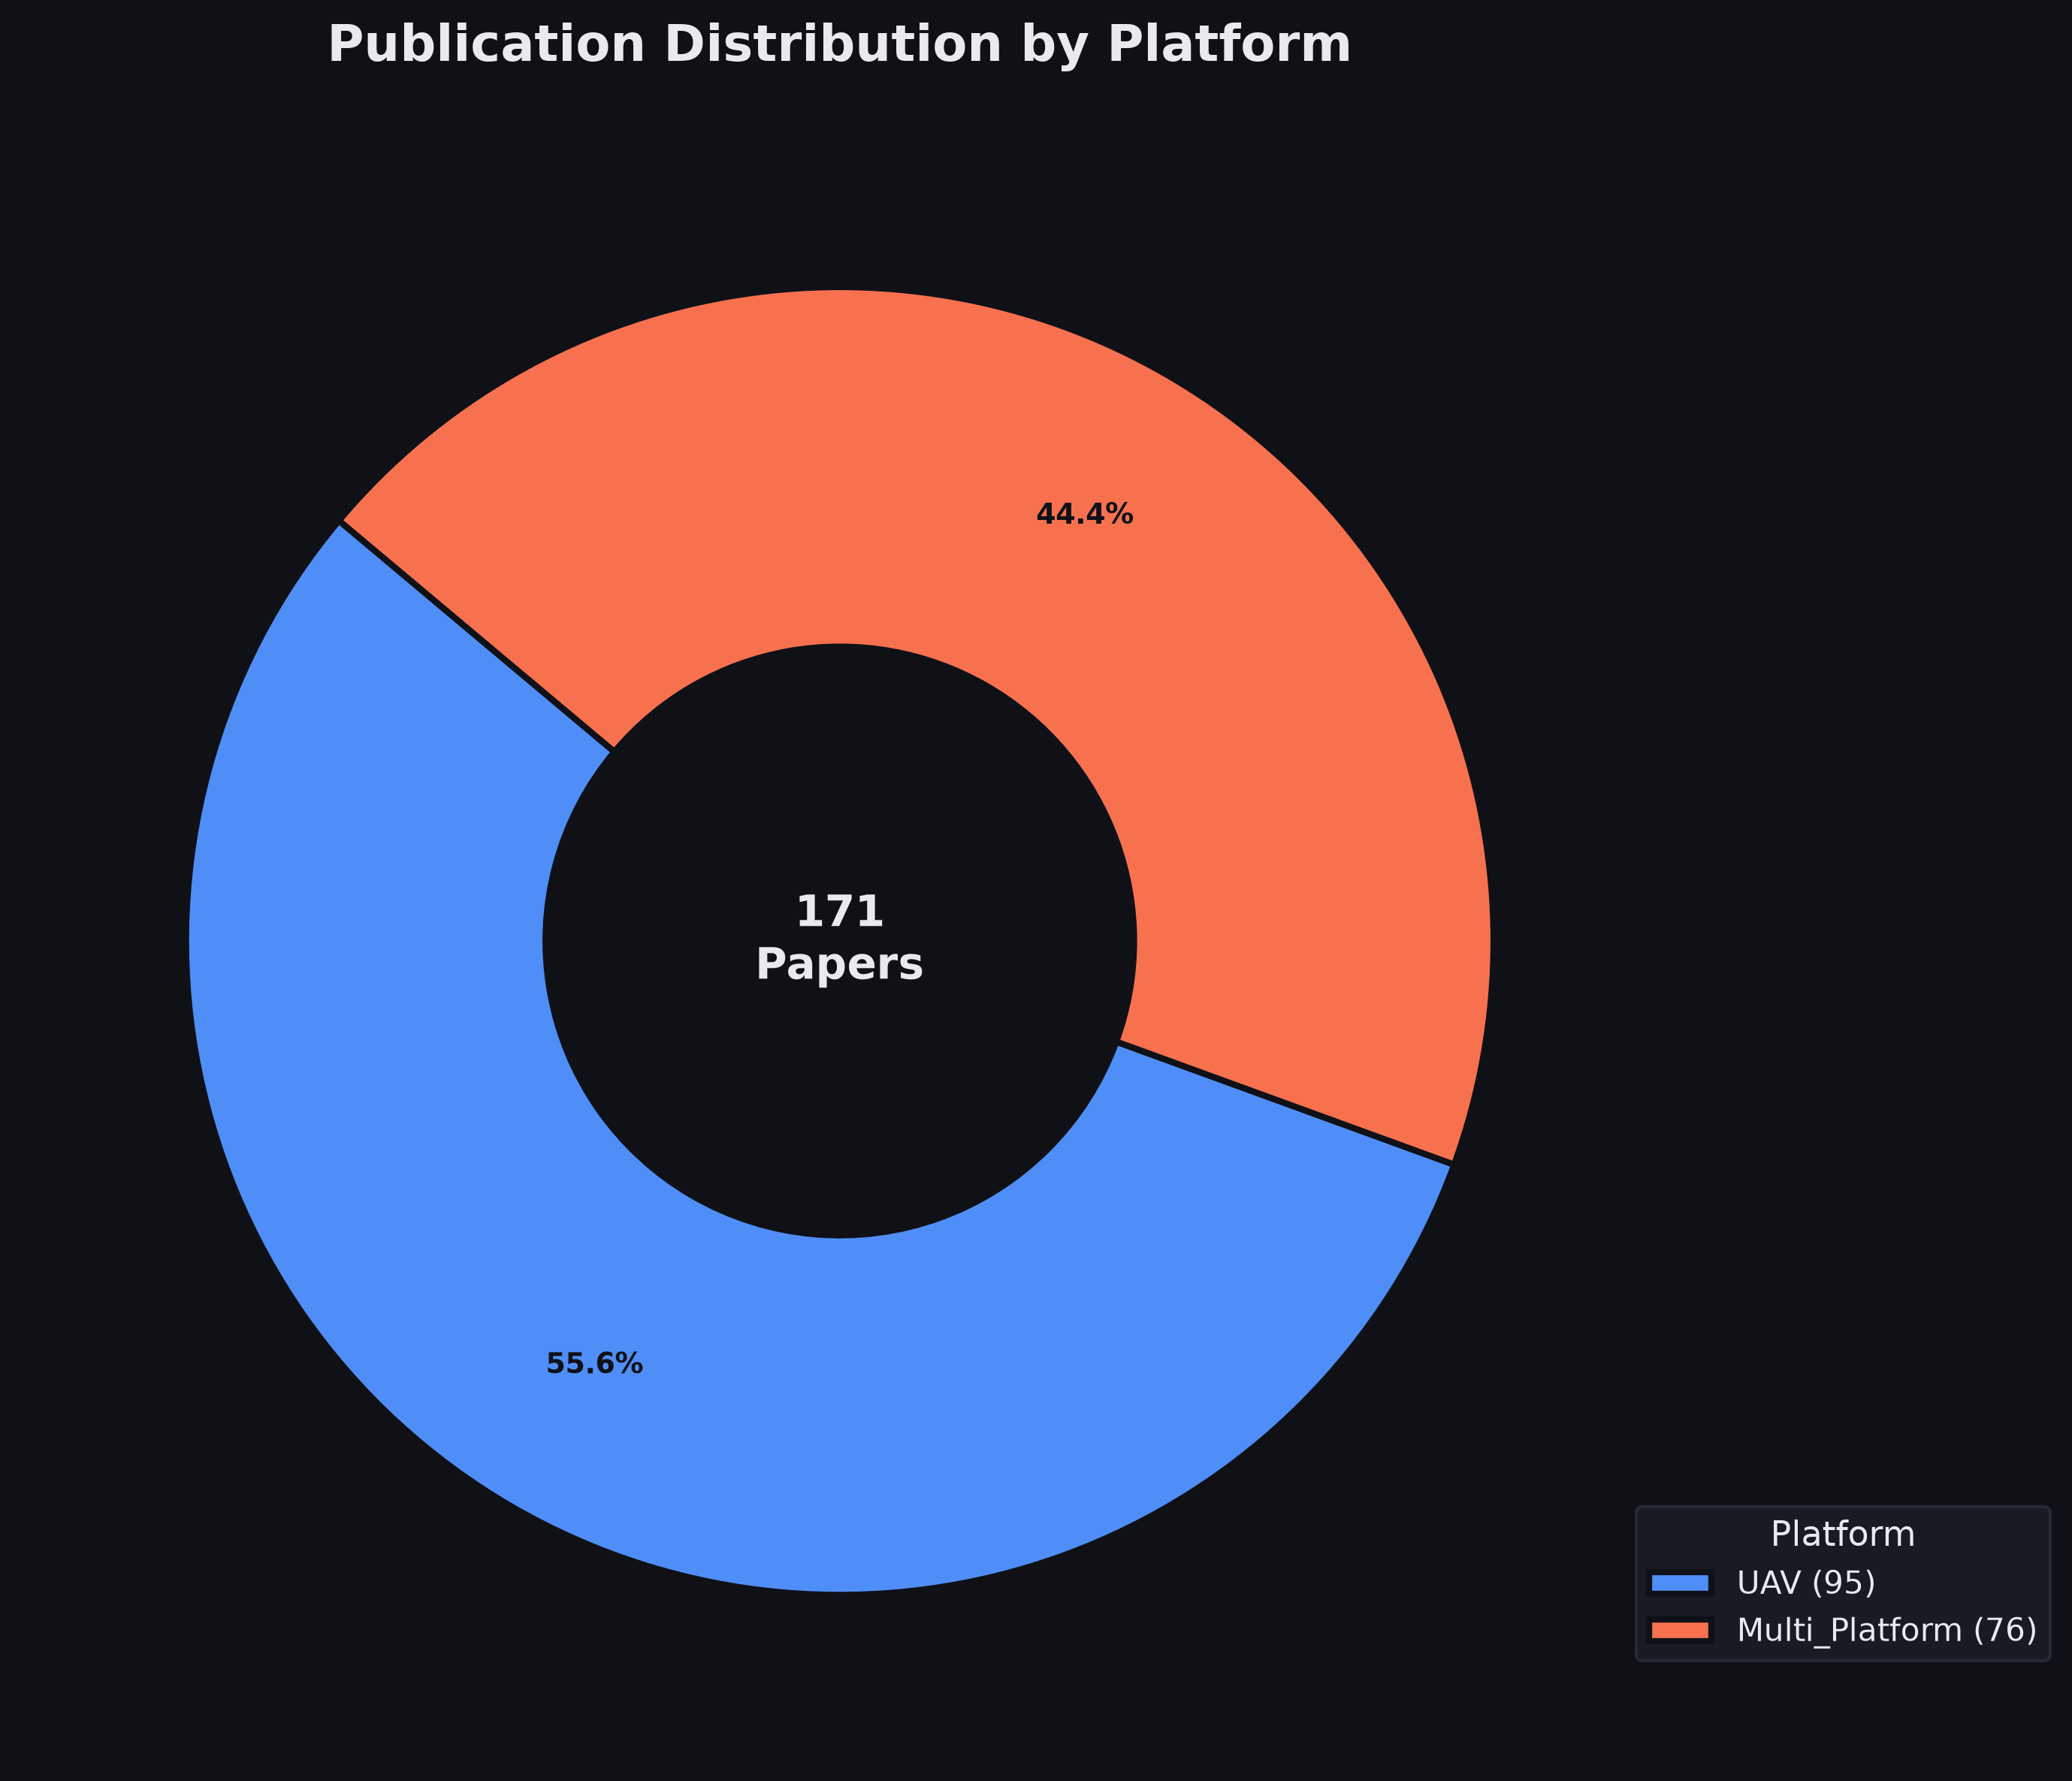
\includegraphics[width=\columnwidth]{../06_analysis/output/figures_v2/fig02_platform_distribution.png}
\caption{Platform distribution.}
\label{fig2}
\end{figure}

\begin{figure}[htbp]
\centering
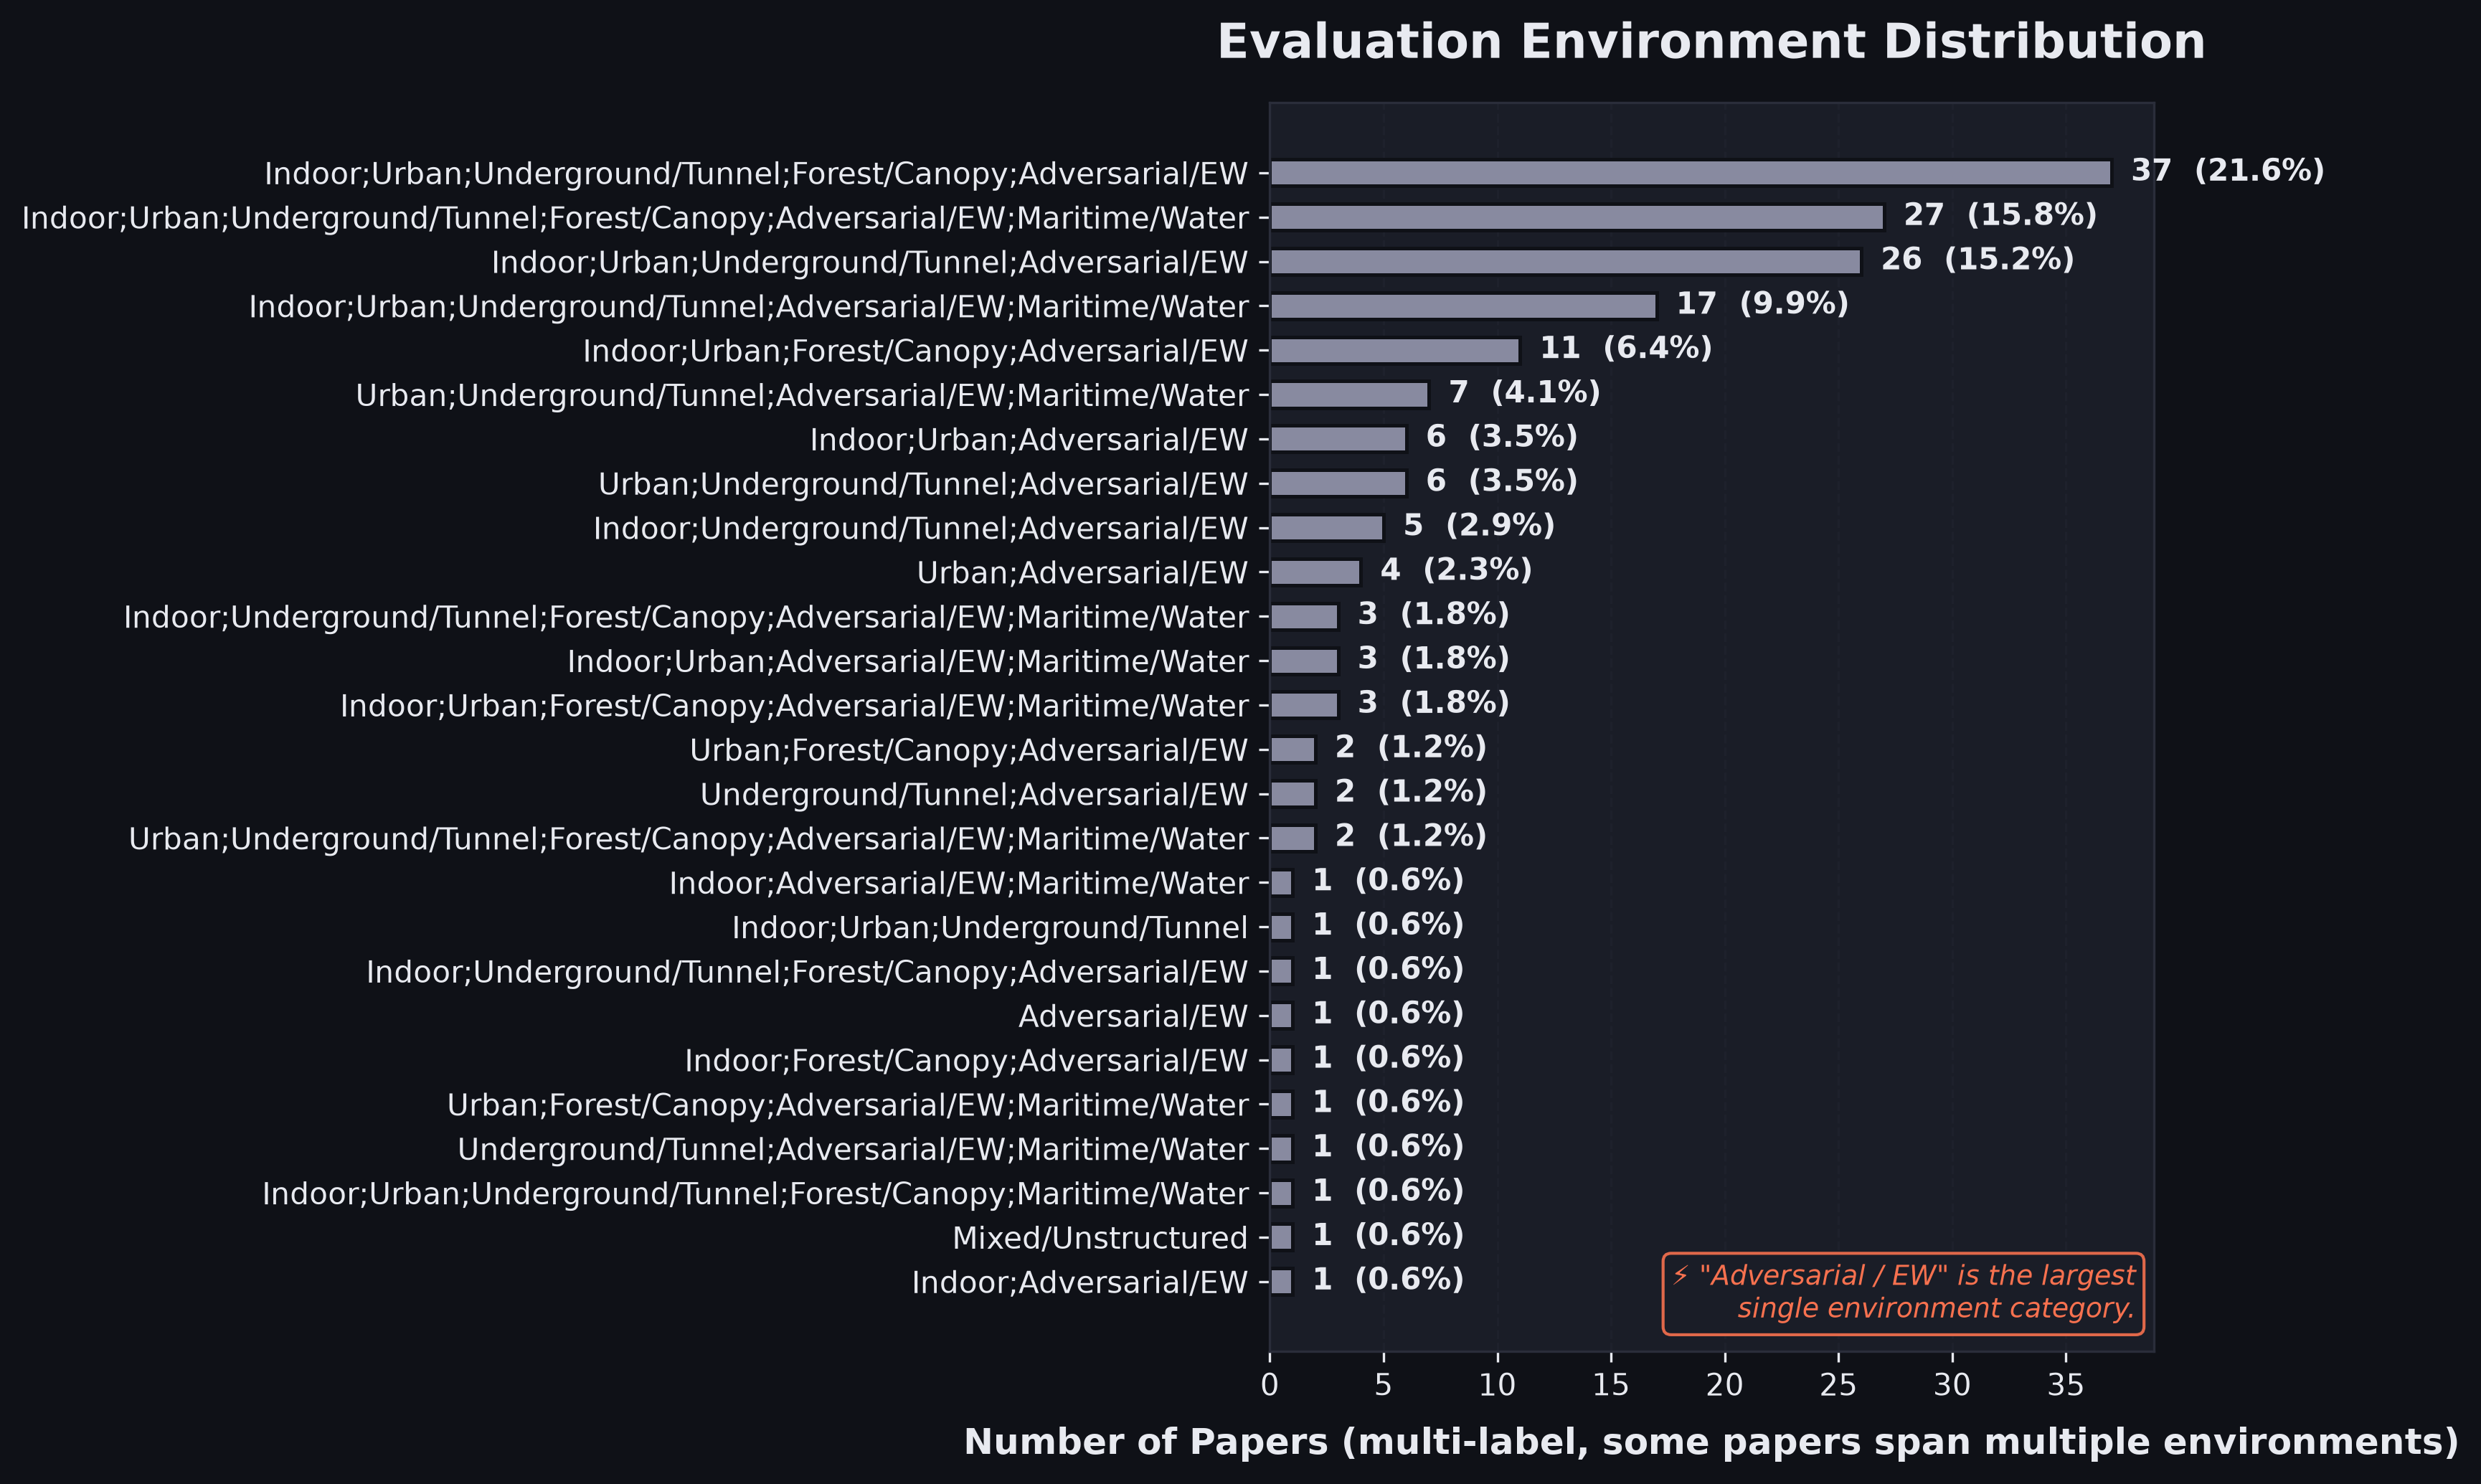
\includegraphics[width=\columnwidth]{../06_analysis/output/figures_v2/fig03_environment_distribution.png}
\caption{Environment distribution with QA tiers.}
\label{fig3}
\end{figure}

\begin{figure}[htbp]
\centering
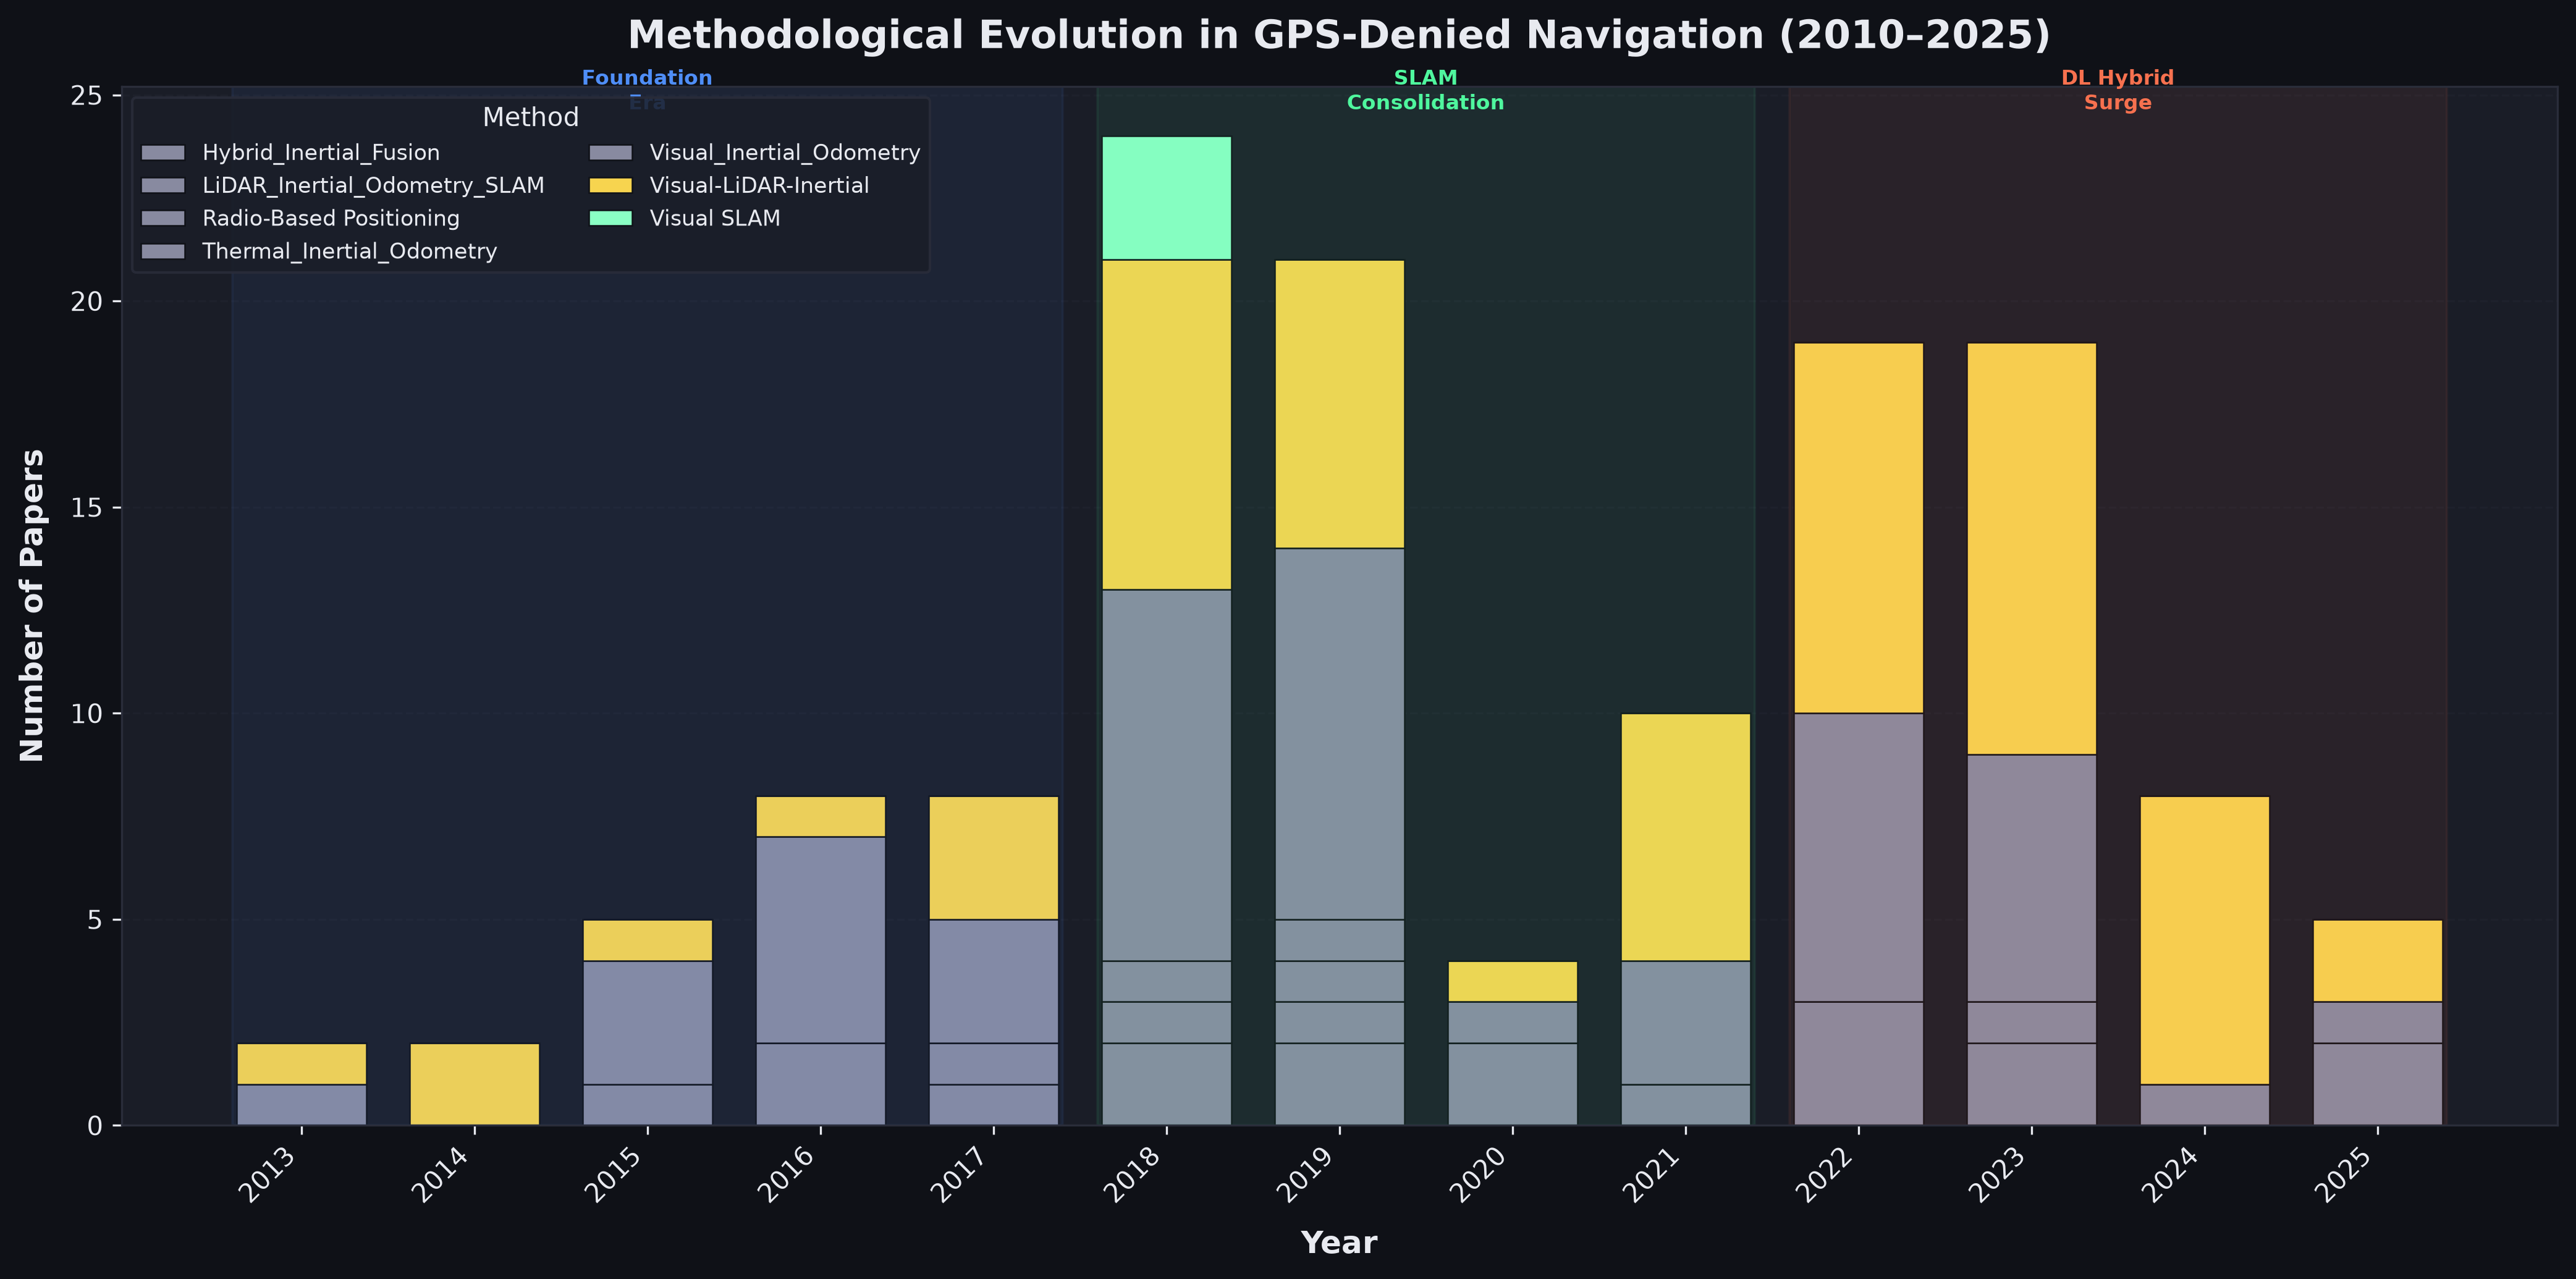
\includegraphics[width=\columnwidth]{../06_analysis/output/figures_v2/fig04_method_evolution.png}
\caption{Method evolution.}
\label{fig4}
\end{figure}

\begin{figure}[htbp]
\centering
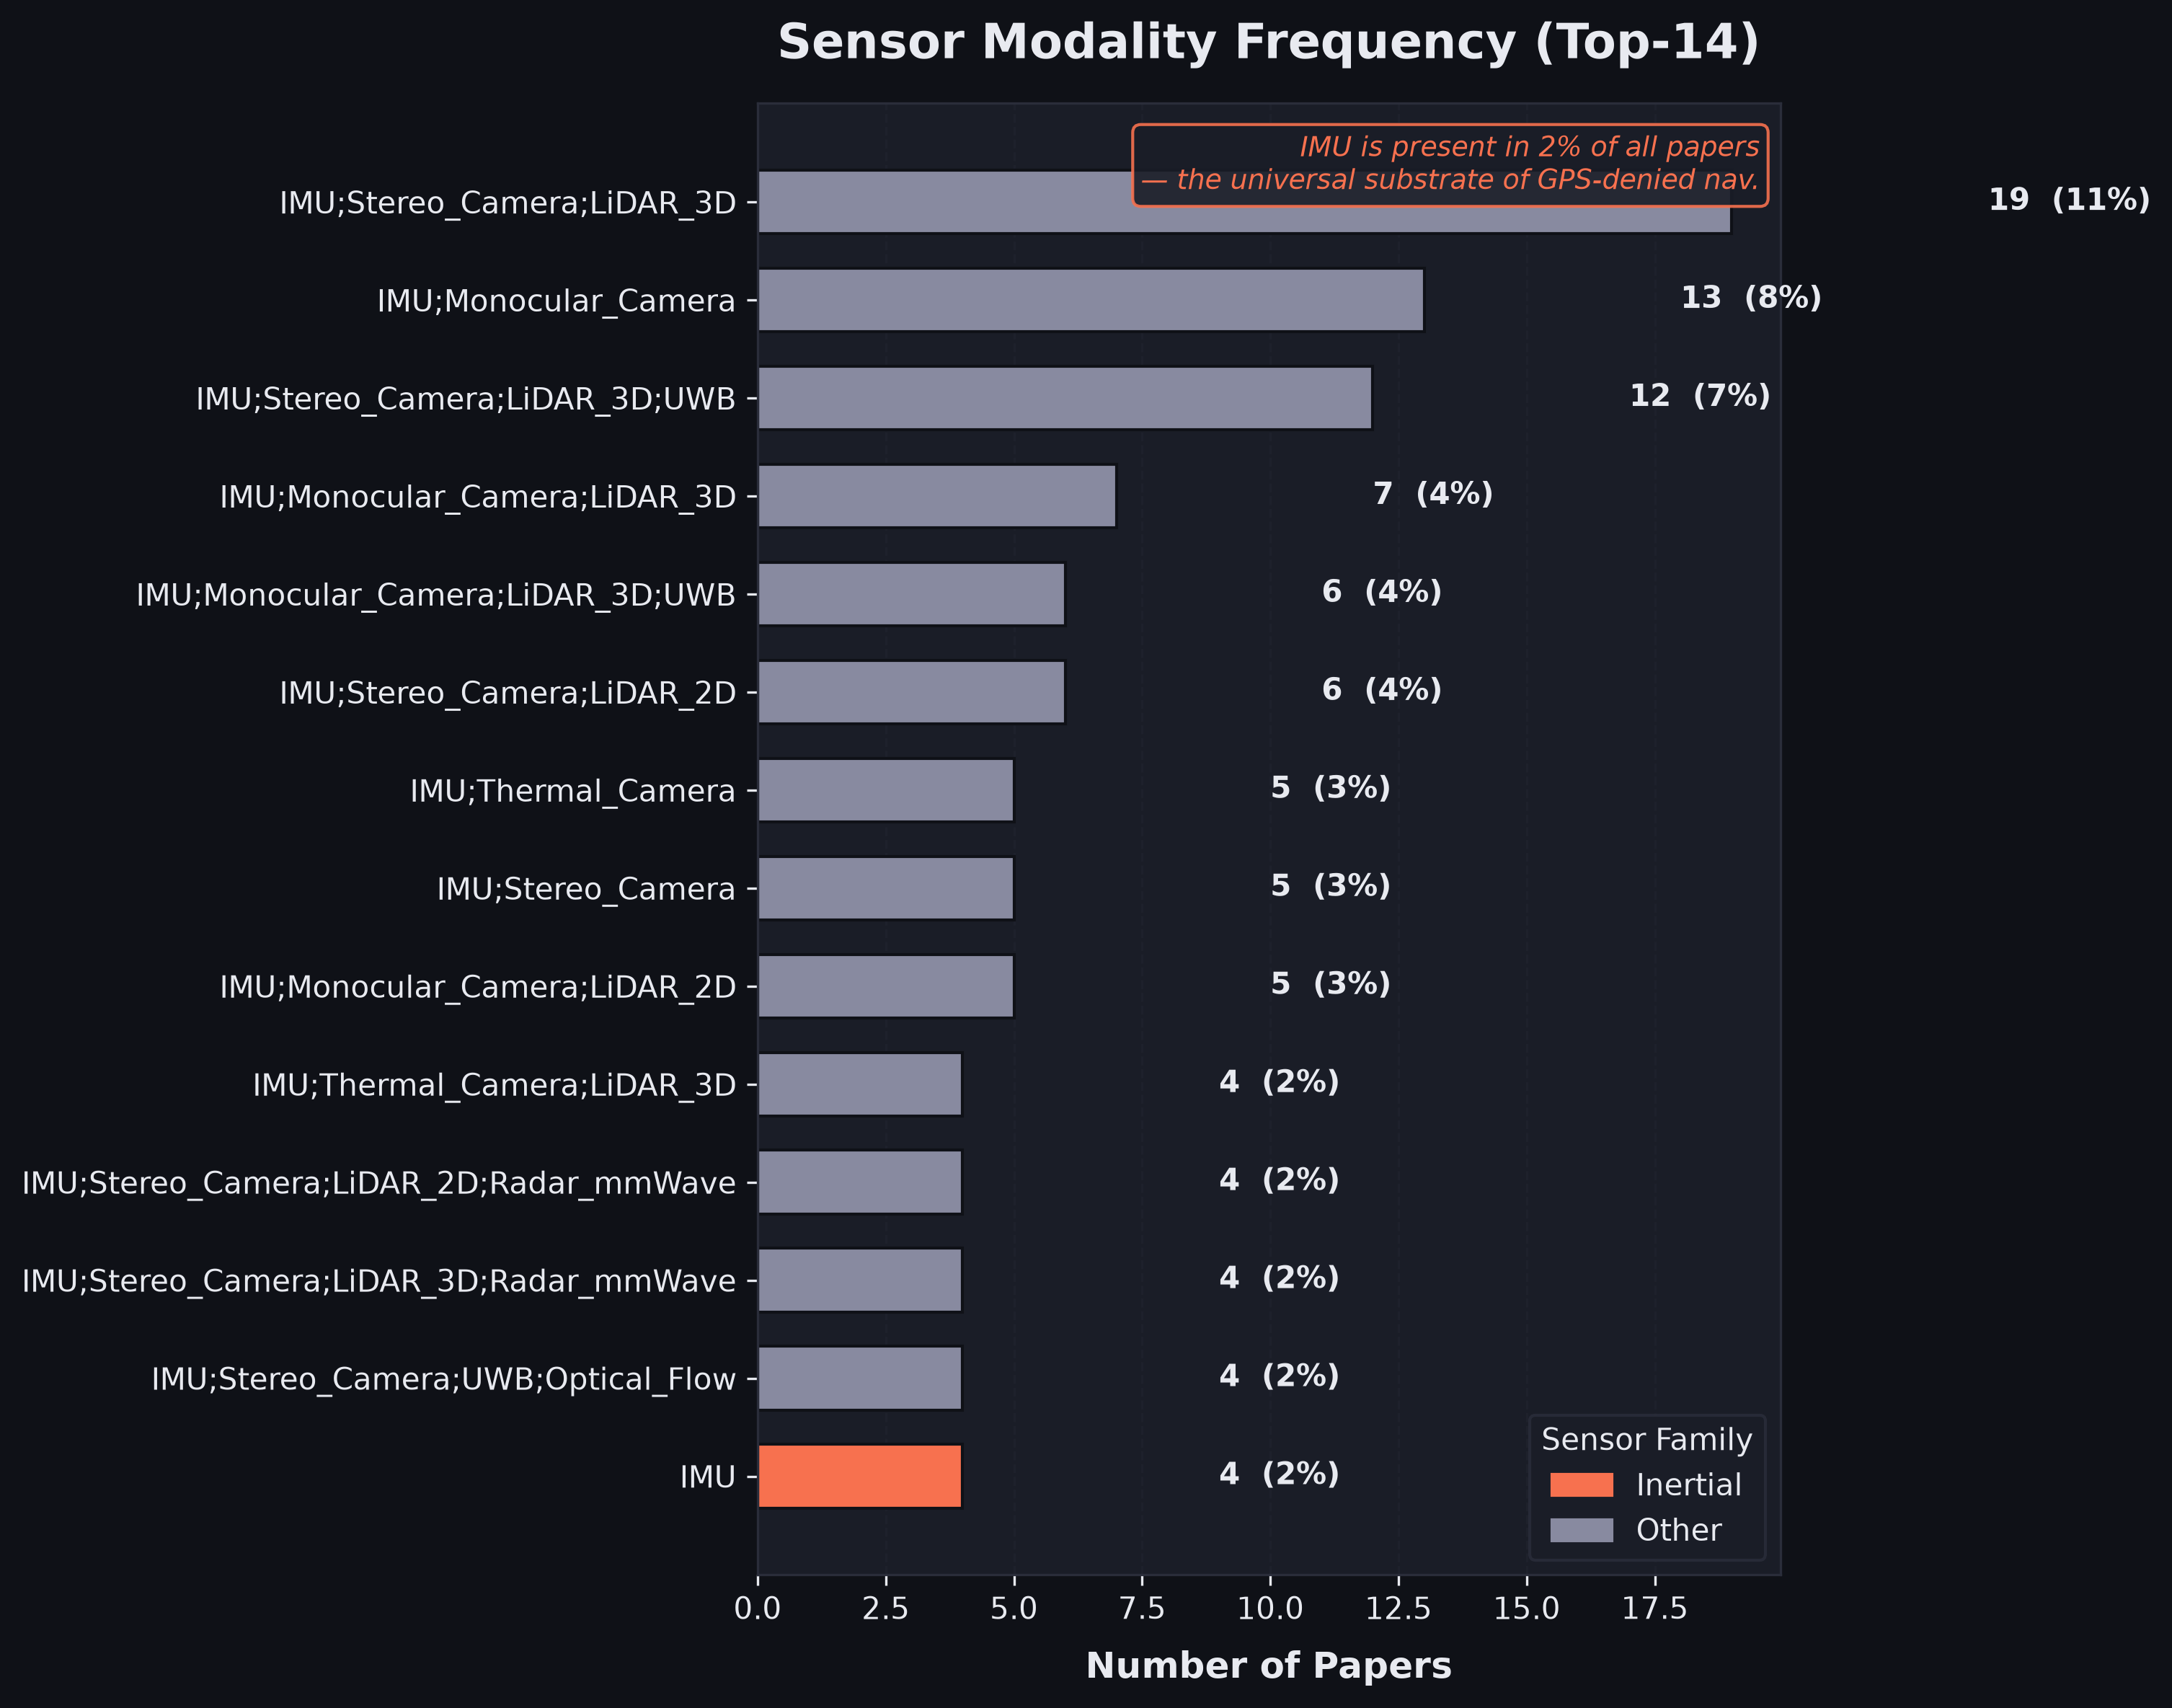
\includegraphics[width=\columnwidth]{../06_analysis/output/figures_v2/fig05_sensor_frequency.png}
\caption{Sensor frequency.}
\label{fig5}
\end{figure}

\begin{figure}[htbp]
\centering
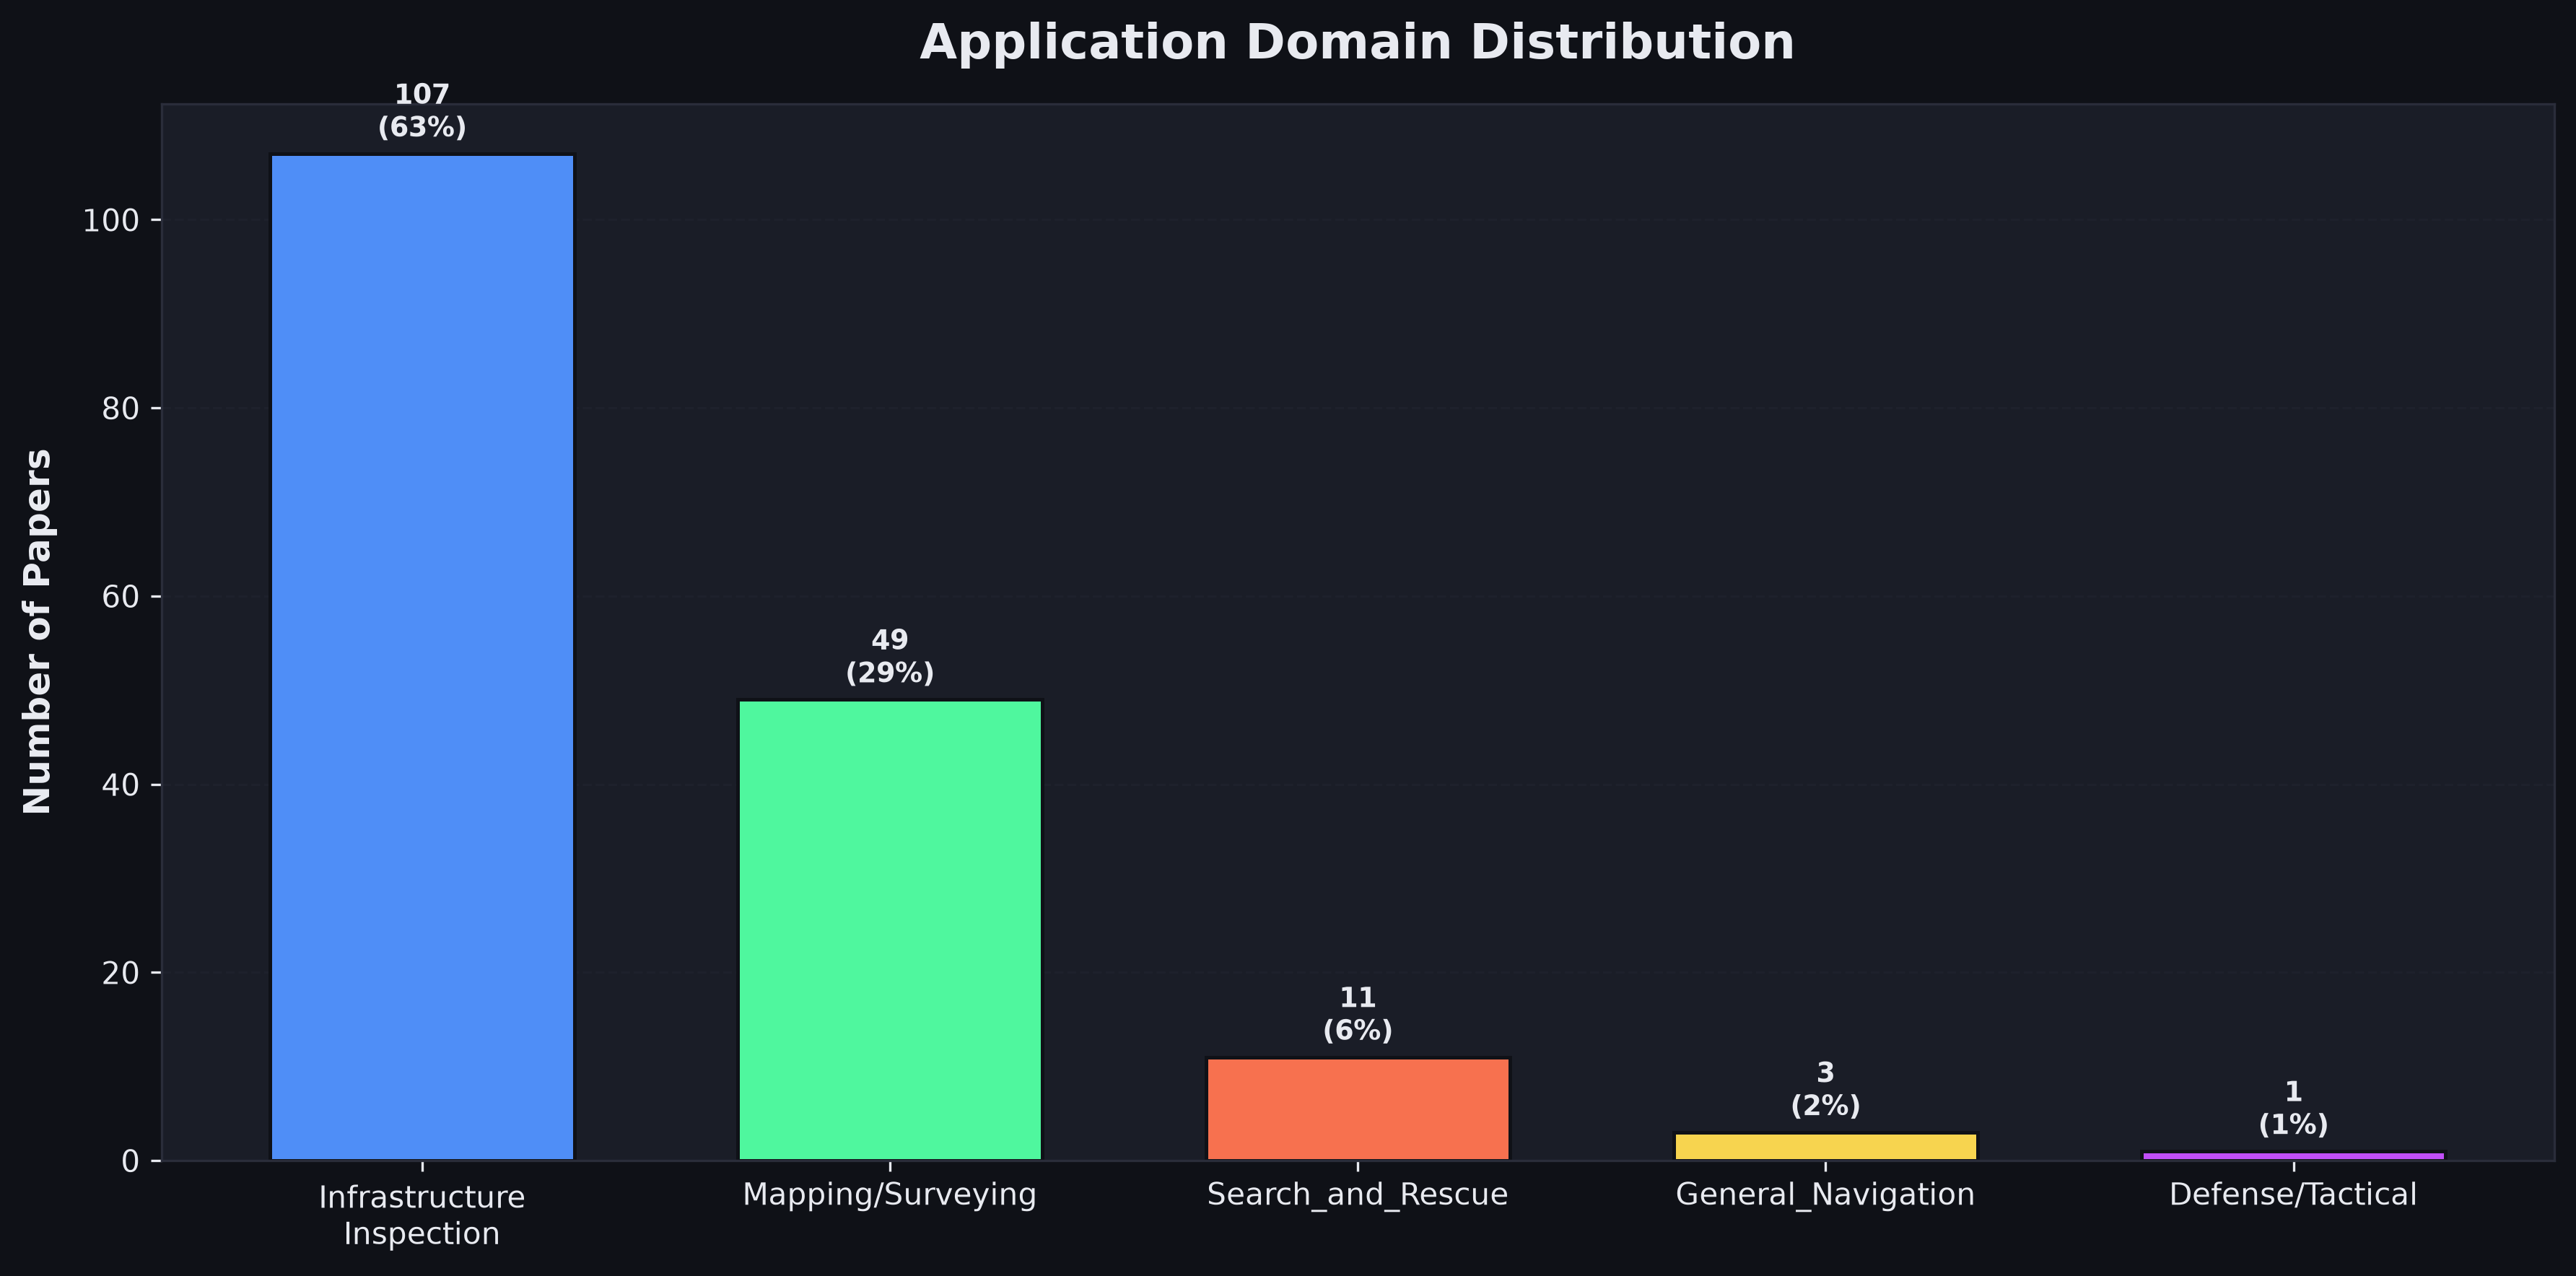
\includegraphics[width=\columnwidth]{../06_analysis/output/figures_v2/fig06_application_domains.png}
\caption{Application domains.}
\label{fig6}
\end{figure}

\begin{figure}[htbp]
\centering
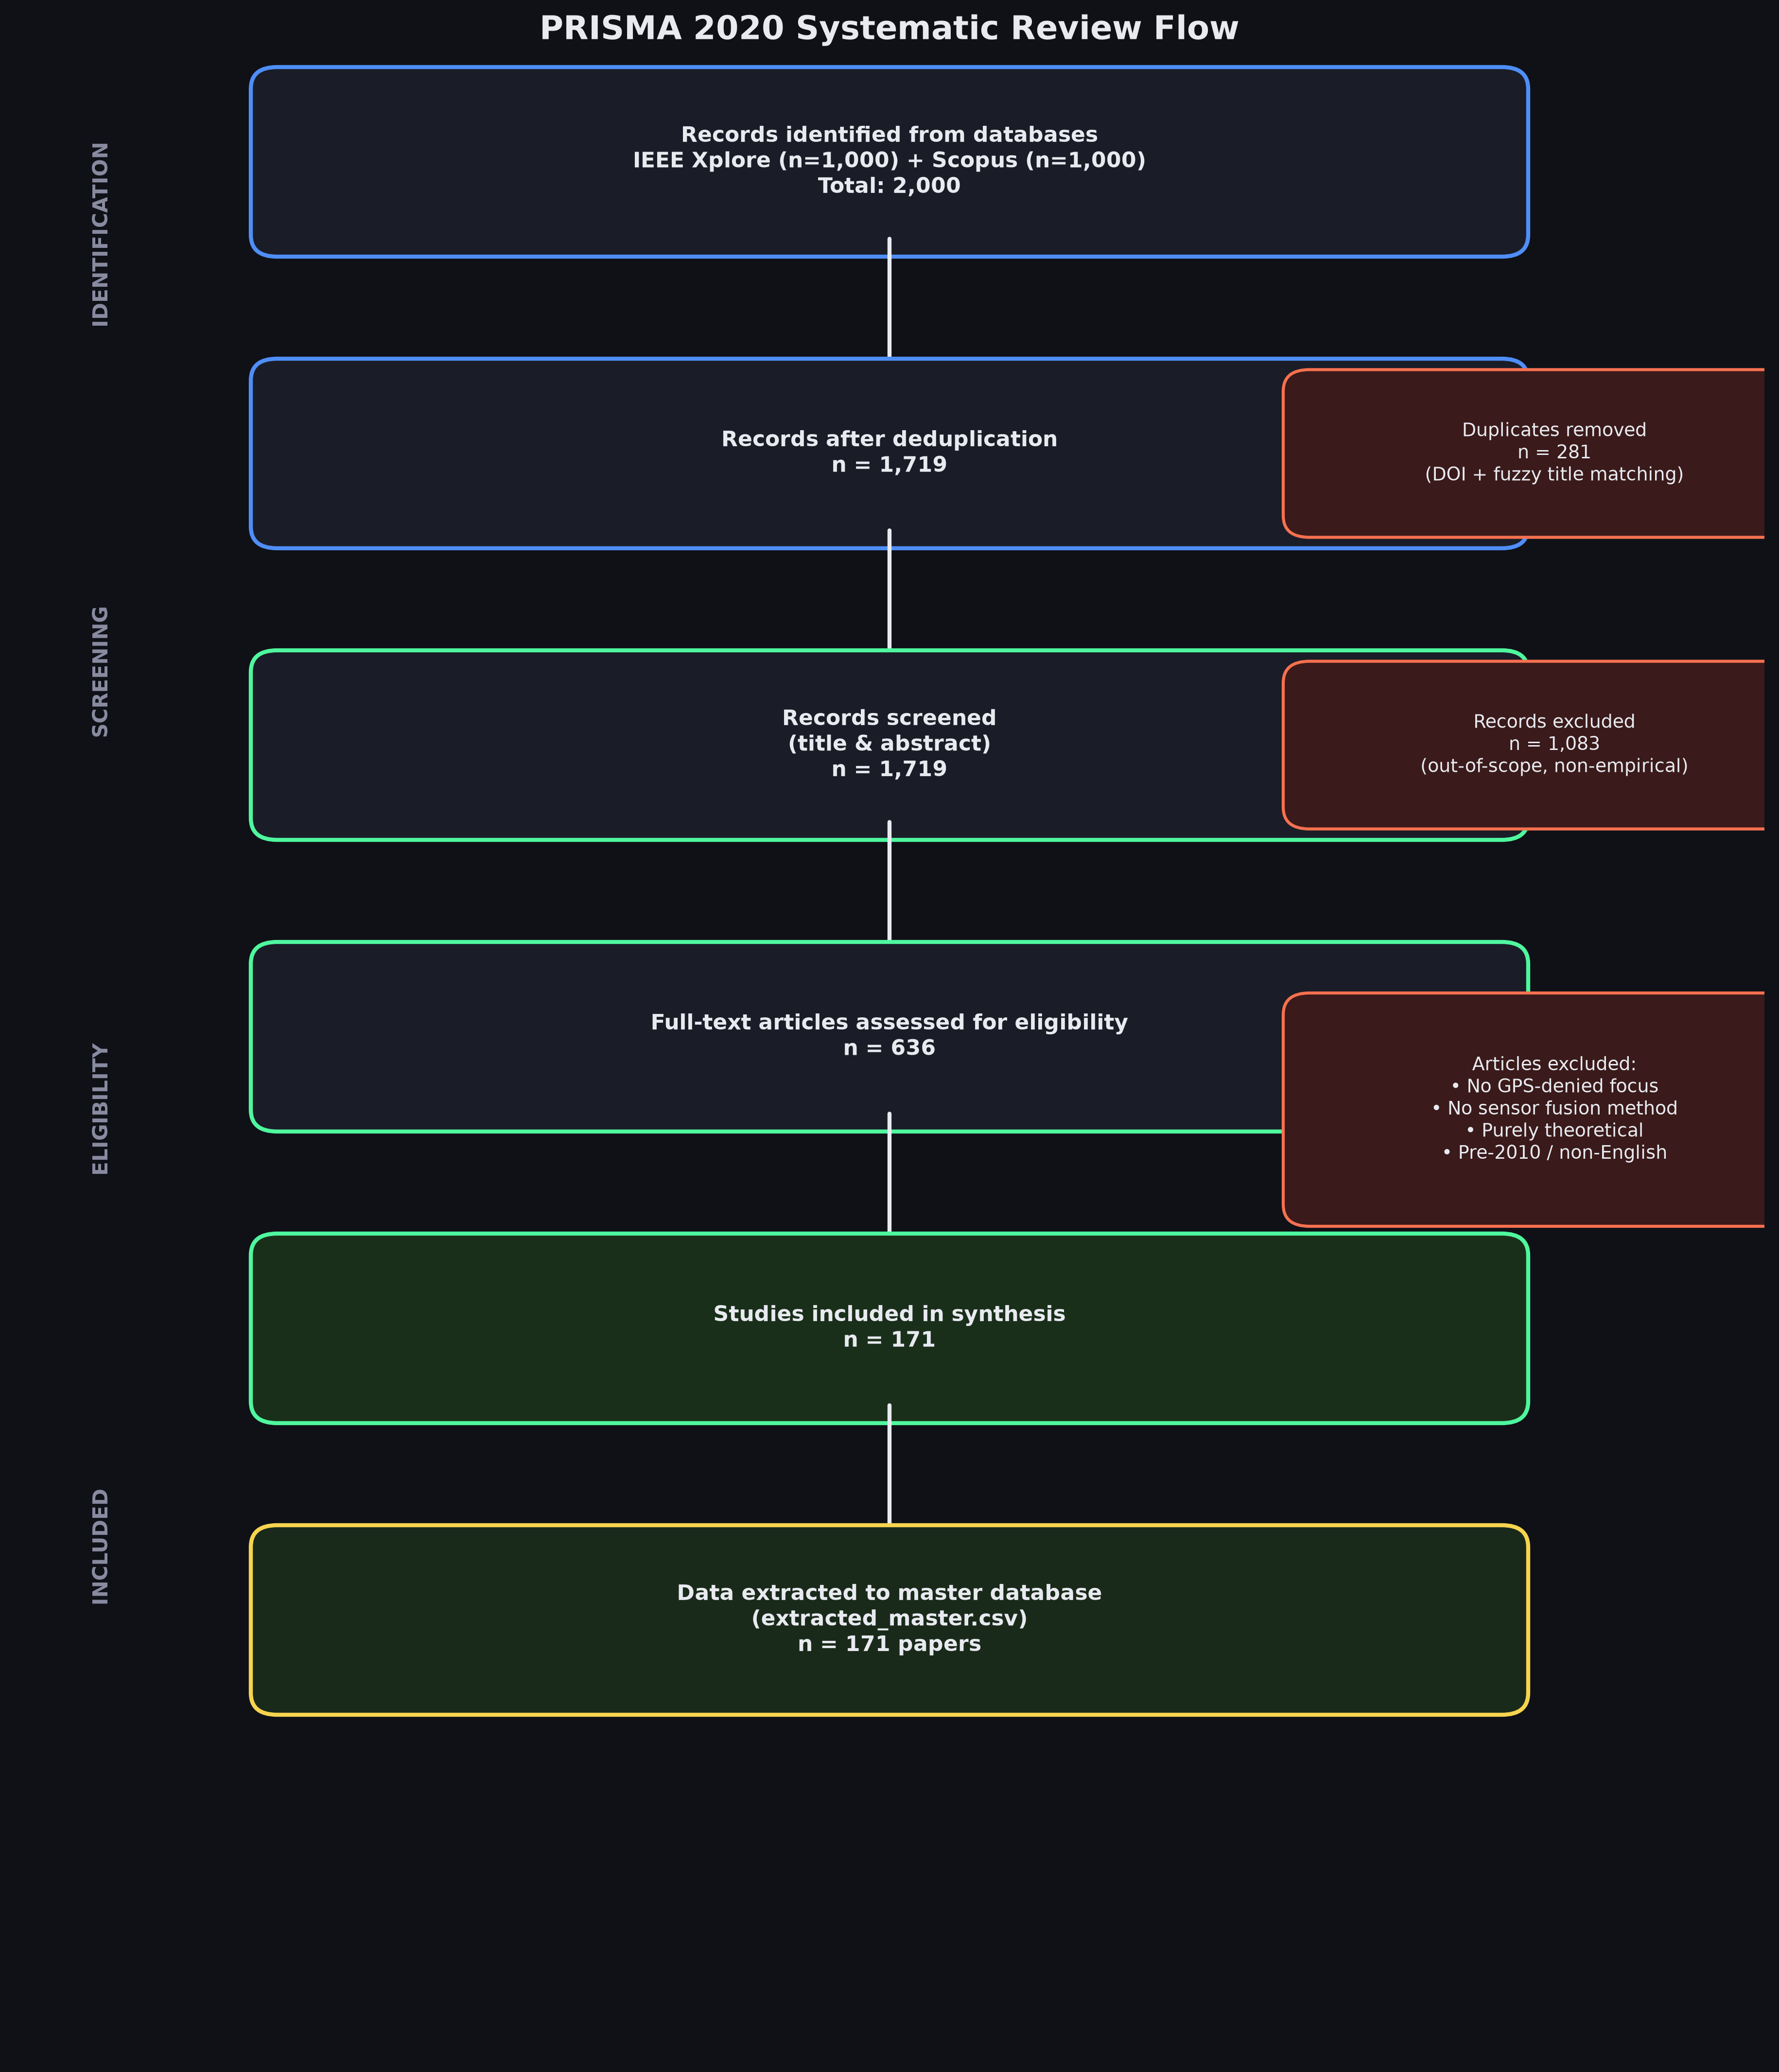
\includegraphics[width=\columnwidth]{../06_analysis/output/figures_v2/fig07_prisma_flow.png}
\caption{PRISMA flow chart.}
\label{fig7}
\end{figure}

\begin{figure}[htbp]
\centering
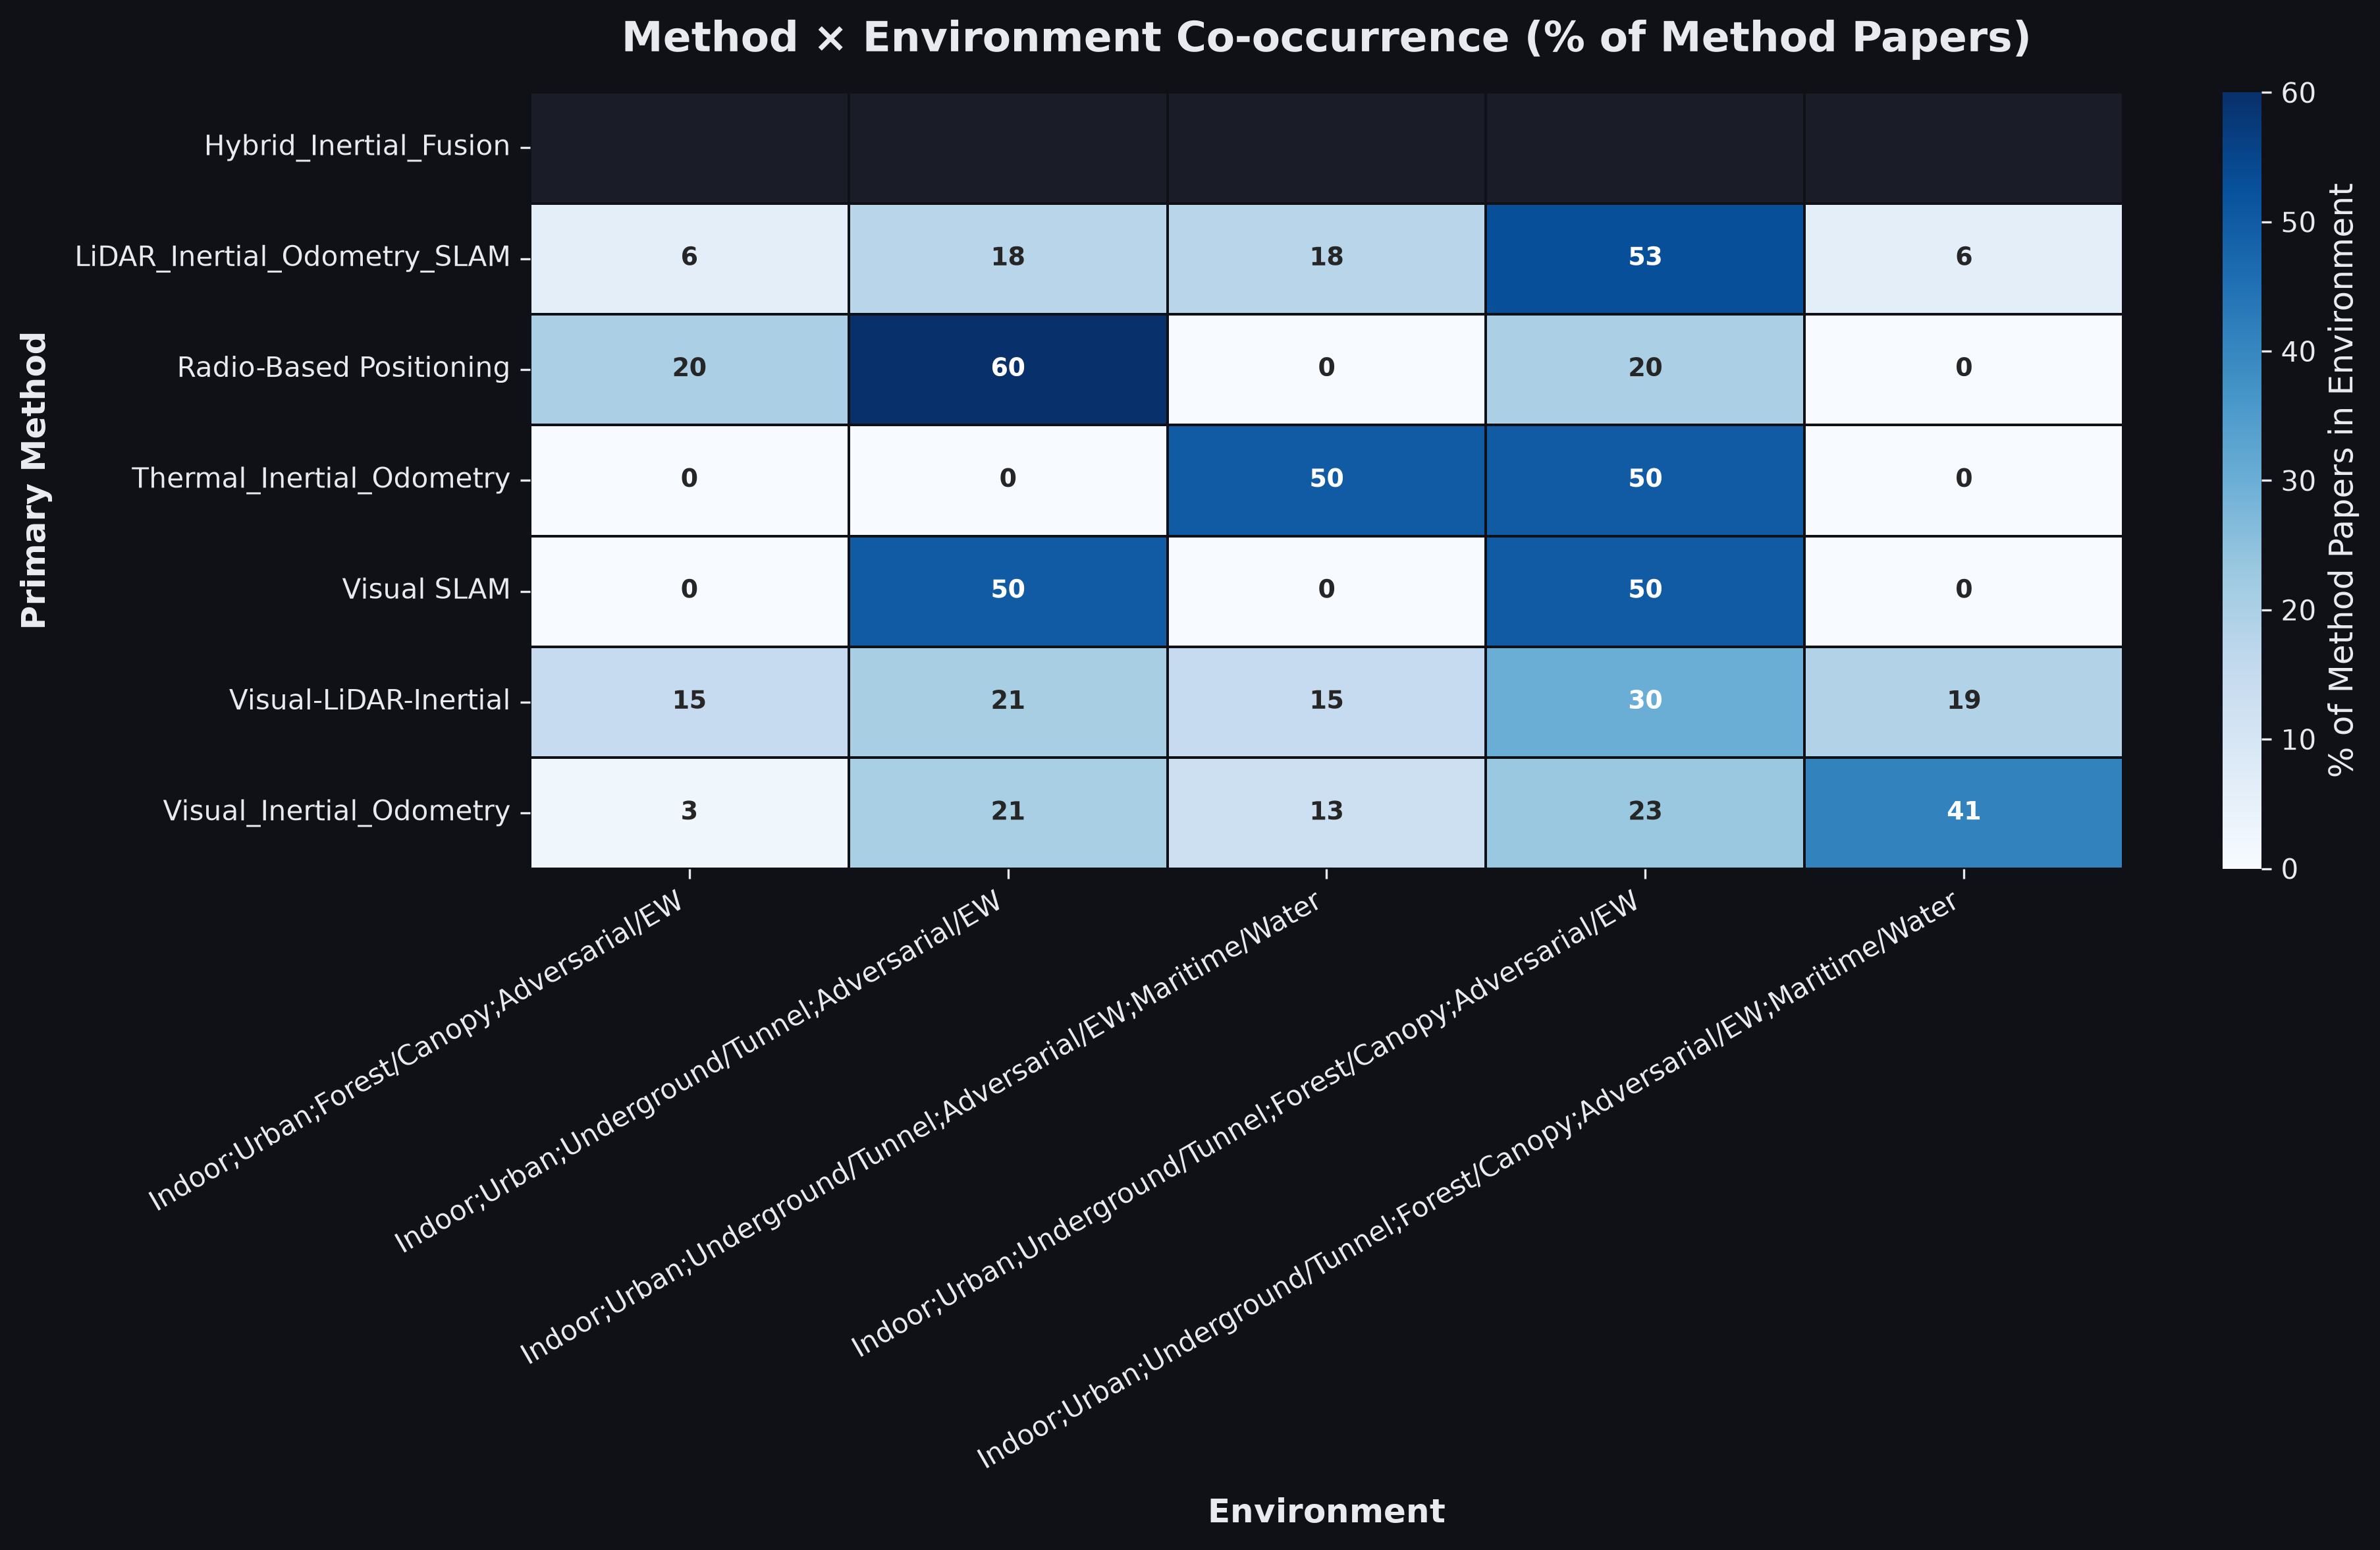
\includegraphics[width=\columnwidth]{../06_analysis/output/figures_v2/fig08_method_environment_heatmap.png}
\caption{Method environment heatmap.}
\label{fig8}
\end{figure}

\begin{figure}[htbp]
\centering
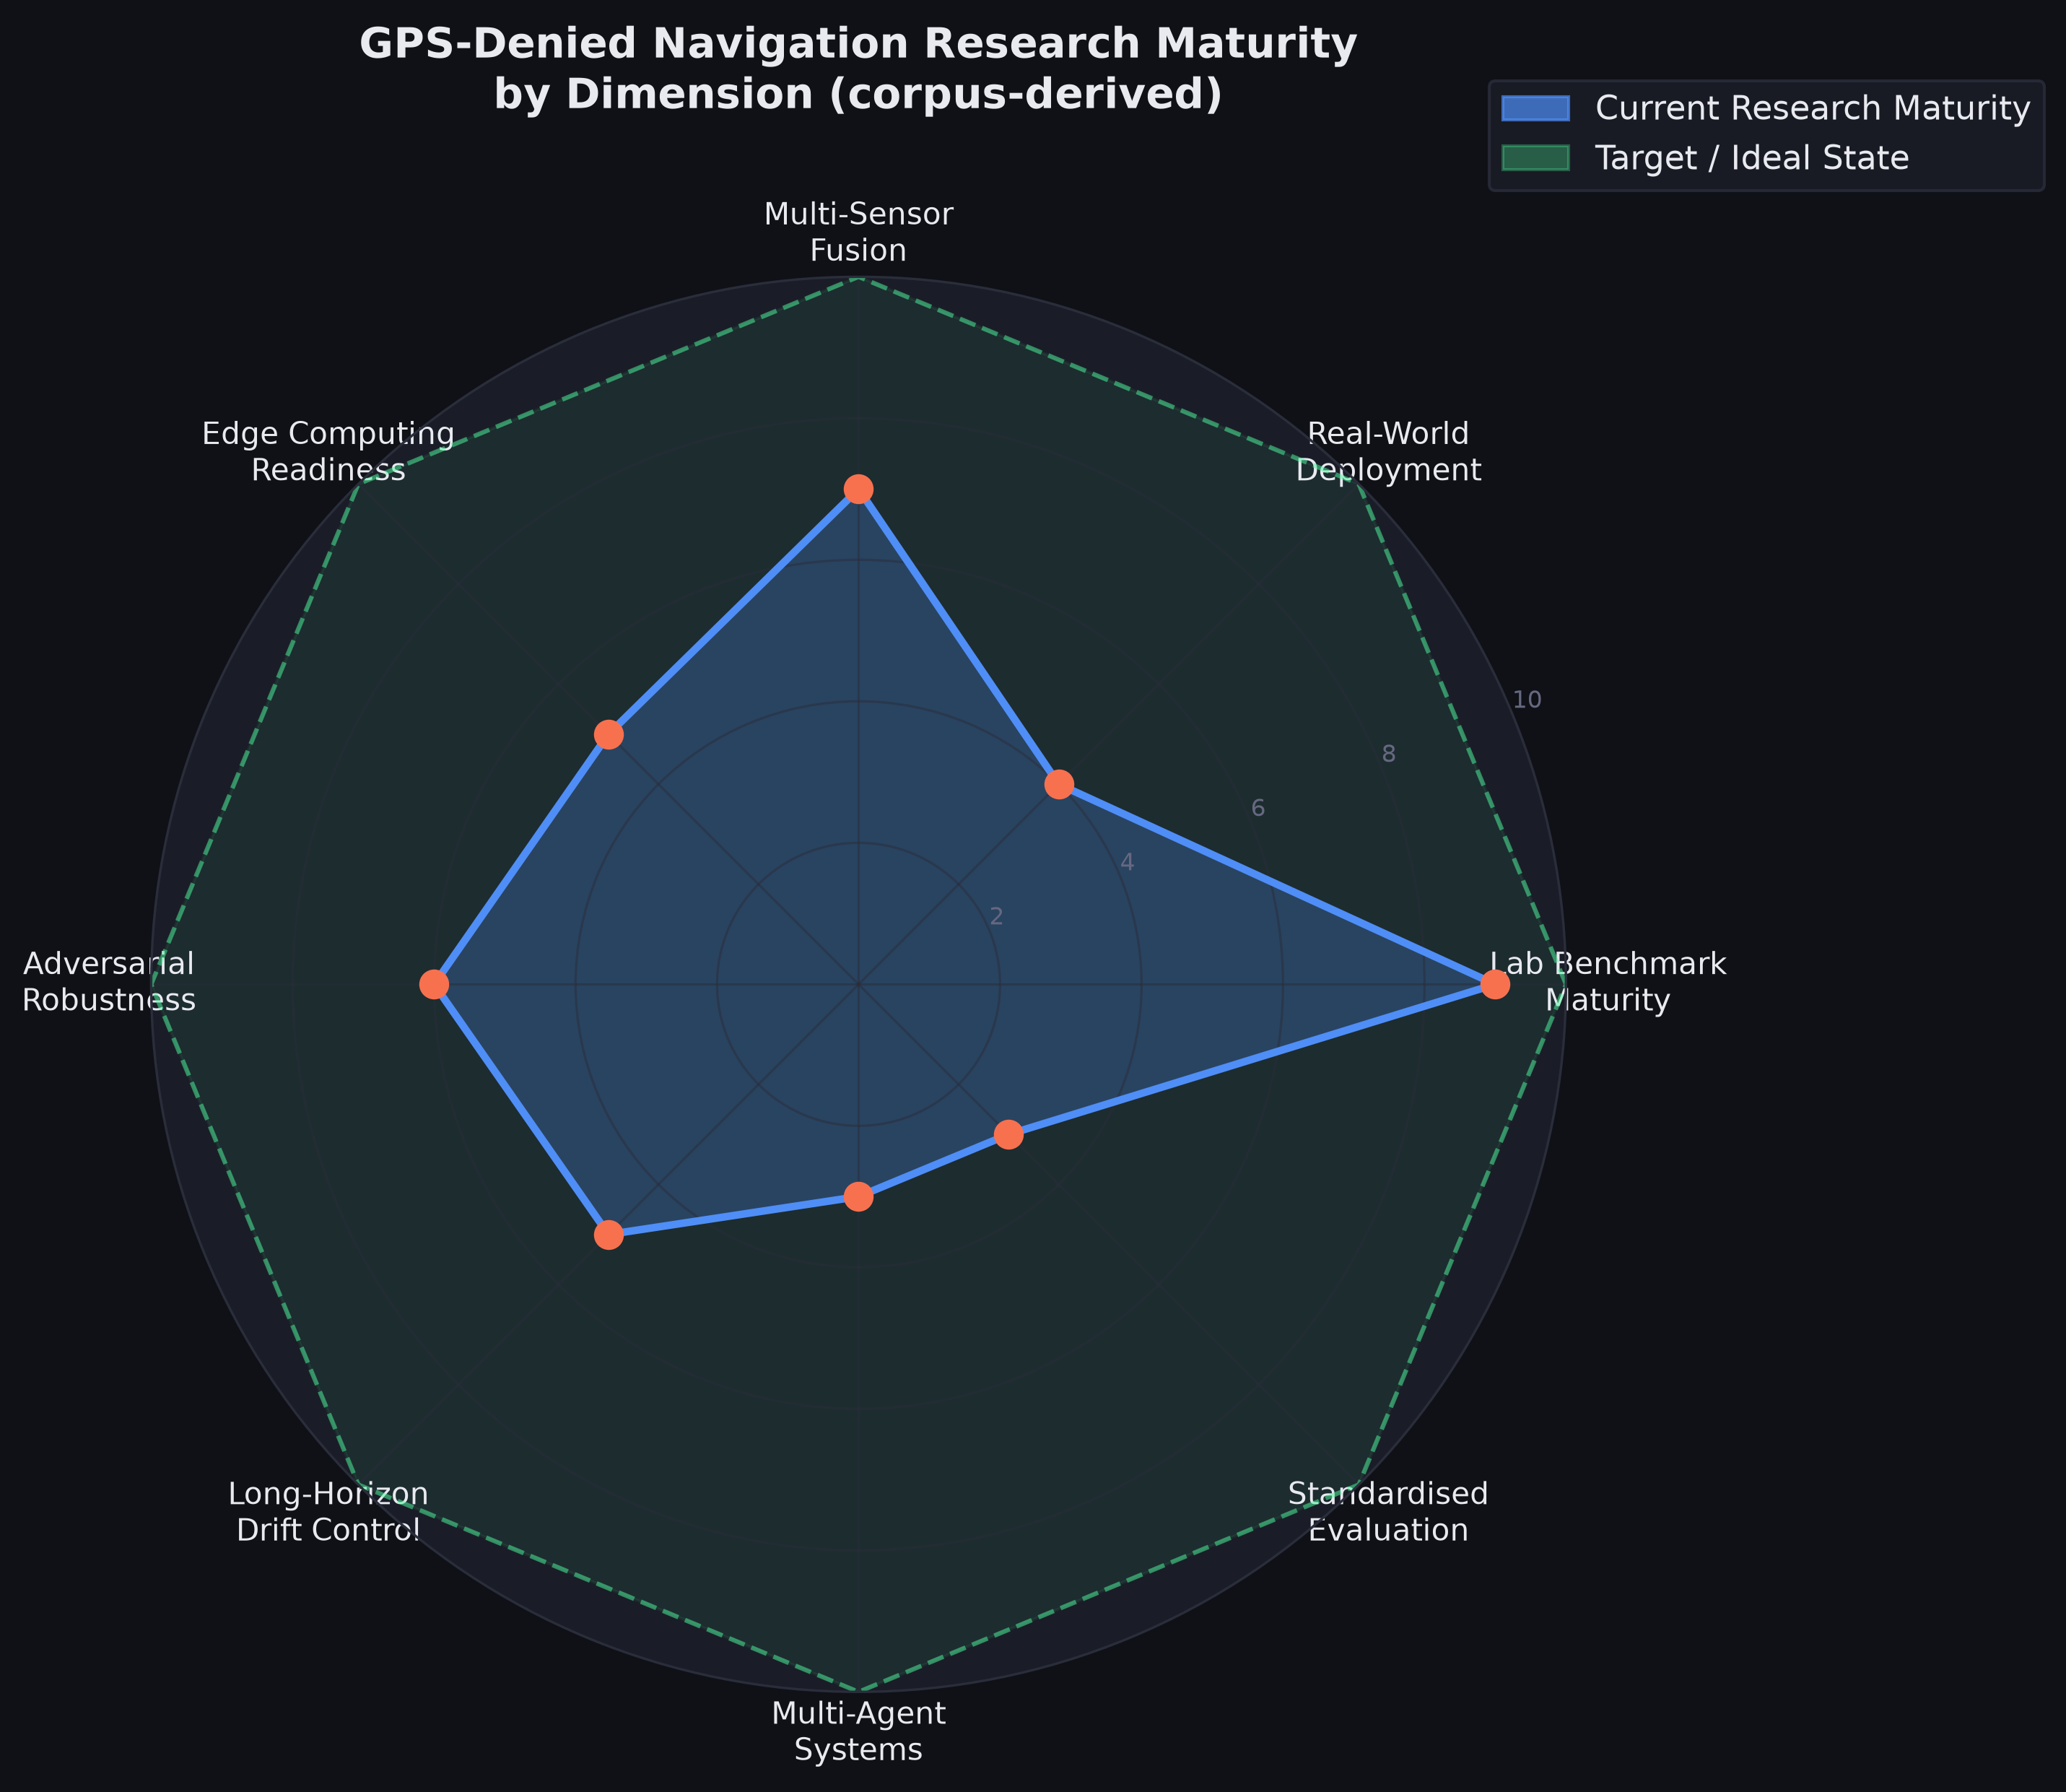
\includegraphics[width=\columnwidth]{../06_analysis/output/figures_v2/fig09_research_maturity_radar.png}
\caption{Maturity radar with QA tiers.}
\label{fig9}
\end{figure}

\section{Conclusion}
Conclusion text.

\bibliographystyle{IEEEtran}
\bibliography{references}

\end{document}
